\documentclass[journal,12pt,twocolumn]{IEEEtran}
\usepackage{setspace}
\usepackage{gensymb}
\usepackage{xcolor}
\usepackage{caption}
\singlespacing
\usepackage{siunitx}
\usepackage[cmex10]{amsmath}
\usepackage{mathtools}
\usepackage{hyperref}
\usepackage{amsthm}
\usepackage{mathrsfs}
\usepackage{txfonts}
\usepackage{stfloats}
\usepackage{cite}
\usepackage{cases}
\usepackage{subfig}
\usepackage{longtable}
\usepackage{multirow}
\usepackage{enumitem}
\usepackage{mathtools}
\usepackage{listings}
\usepackage{tikz}
\usetikzlibrary{shapes,arrows,positioning}
\usepackage{circuitikz}
\let\vec\mathbf
\DeclareMathOperator*{\Res}{Res}
\renewcommand\thesection{\arabic{section}}
\renewcommand\thesubsection{\thesection.\arabic{subsection}}
\renewcommand\thesubsubsection{\thesubsection.\arabic{subsubsection}}

\renewcommand\thesectiondis{\arabic{section}}
\renewcommand\thesubsectiondis{\thesectiondis.\arabic{subsection}}
\renewcommand\thesubsubsectiondis{\thesubsectiondis.\arabic{subsubsection}}
\hyphenation{op-tical net-works semi-conduc-tor}

\lstset{
language=Python,
frame=single, 
breaklines=true,
columns=fullflexible
}
\begin{document}
\theoremstyle{definition}
\newtheorem{theorem}{Theorem}[section]
\newtheorem{problem}{Problem}
\newtheorem{proposition}{Proposition}[section]
\newtheorem{lemma}{Lemma}[section]
\newtheorem{corollary}[theorem]{Corollary}
\newtheorem{example}{Example}[section]
\newtheorem{definition}{Definition}[section]
\newcommand{\BEQA}{\begin{eqnarray}}
\newcommand{\EEQA}{\end{eqnarray}}
\newcommand{\define}{\stackrel{\triangle}{=}}
\newenvironment{amatrix}[1]{%
  \left(\begin{array}{@{}*{#1}{c}|c@{}}
}{%
  \end{array}\right)
}
\newcommand{\myvec}[1]{\ensuremath{\begin{pmatrix}#1\end{pmatrix}}}
\newcommand{\myaugvec}[2]{\ensuremath{\begin{amatrix}{#1}#2\end{amatrix}}}
\newcommand{\mydet}[1]{\ensuremath{\begin{vmatrix}#1\end{vmatrix}}}
\bibliographystyle{IEEEtran}
\providecommand{\nCr}[2]{\,^{#1}C_{#2}} % nCr
\providecommand{\nPr}[2]{\,^{#1}P_{#2}} % nPr
\providecommand{\mbf}{\mathbf}
\providecommand{\pr}[1]{\ensuremath{\Pr\left(#1\right)}}
\providecommand{\qfunc}[1]{\ensuremath{Q\left(#1\right)}}
\providecommand{\sbrak}[1]{\ensuremath{{}\left[#1\right]}}
\providecommand{\lsbrak}[1]{\ensuremath{{}\left[#1\right.}}
\providecommand{\rsbrak}[1]{\ensuremath{{}\left.#1\right]}}
\providecommand{\brak}[1]{\ensuremath{\left(#1\right)}}
\providecommand{\lbrak}[1]{\ensuremath{\left(#1\right.}}
\providecommand{\rbrak}[1]{\ensuremath{\left.#1\right)}}
\providecommand{\cbrak}[1]{\ensuremath{\left\{#1\right\}}}
\providecommand{\lcbrak}[1]{\ensuremath{\left\{#1\right.}}
\providecommand{\rcbrak}[1]{\ensuremath{\left.#1\right\}}}
\theoremstyle{remark}
\newtheorem{rem}{Remark}
\newcommand{\sgn}{\mathop{\mathrm{sgn}}}
\newcommand{\rect}{\mathop{\mathrm{rect}}}
\newcommand{\sinc}{\mathop{\mathrm{sinc}}}
\providecommand{\abs}[1]{\left\vert#1\right\vert}
\providecommand{\res}[1]{\Res\displaylimits_{#1}} 
\providecommand{\norm}[1]{\left\Vert#1\right\Vert}
\providecommand{\mtx}[1]{\mathbf{#1}}
\providecommand{\mean}[1]{E\left[ #1 \right]}
\providecommand{\fourier}{\overset{\mathcal{F}}{ \rightleftharpoons}}
\providecommand{\ztrans}{\overset{\mathcal{Z}}{ \rightleftharpoons}}
\providecommand{\system}[1]{\overset{\mathcal{#1}}{ \longleftrightarrow}}
\newcommand{\solution}{\noindent \textbf{Solution: }}
\providecommand{\dec}[2]{\ensuremath{\overset{#1}{\underset{#2}{\gtrless}}}}
\let\StandardTheFigure\thefigure
\def\putbox#1#2#3{\makebox[0in][l]{\makebox[#1][l]{}\raisebox{\baselineskip}[0in][0in]{\raisebox{#2}[0in][0in]{#3}}}}
     \def\rightbox#1{\makebox[0in][r]{#1}}
     \def\centbox#1{\makebox[0in]{#1}}
     \def\topbox#1{\raisebox{-\baselineskip}[0in][0in]{#1}}
     \def\midbox#1{\raisebox{-0.5\baselineskip}[0in][0in]{#1}}
\numberwithin{equation}{enumi}
\numberwithin{table}{enumi}
\numberwithin{figure}{enumi}
\vspace{3cm}
\title{Chapter 1: Source Coding}
\author{Gautam Singh}
\maketitle
\bigskip

\section{Learning Objective 1}

\begin{enumerate}[label=\thesection.\arabic*, ref=\thesection.\theenumi]
    \item The source entropy is
    \begin{align}
        H(X) &= -\sum_{x\in\mathcal{X}}p(x)\log p(x) \\
        &= 2.23\ \textrm{bits}
        \label{eq:1-1-1}
    \end{align}

    \item The source entropy is
    \begin{align}
        H(X) &= -\sum_{i=1}^{\infty}2^{-i}\brak{-i} \\
        &= \sum_{i=1}^{\infty}\frac{i}{2^i} = 2\ \textrm{bits}
        \label{eq:1-2-1}
    \end{align}

    \item The source entropy is
    \begin{align}
        H(X) &= -\sum_{i=1}^{\infty}p\brak{1-p}^{i-1}\log\brak{p\brak{1-p}^{i-1}} \\
        &= -\brak{\frac{p\log{p}}{1-\brak{1-p}}+\frac{p\log\brak{1-p}\brak{1-p}}{\brak{1-\brak{1-p}}^2}} \\
        &= -\brak{\log{p} + \frac{1-p}{p}\log\brak{1-p}}\ \textrm{bits}
        \label{eq:1-3-1}
    \end{align}

    \item Since $p(H) = p$, we get $p(T) = 1 - p$. Let $E$ denote the event of
    getting at least one head.
    \begin{enumerate}[label=\theenumi.\arabic*, ref=\theenumi.\arabic*]
        \item The probability of failure is clearly $p(E') = \brak{1-p}^N$.
        Hence, the information conveyed by the failure is
        \begin{align}
            I(E') = -N\log\brak{1-p}
            \label{eq:1-4-1}
        \end{align}
        \item When $N \to \infty$ in \eqref{eq:1-4-1}, $I(E') \to \infty$ as
        $0 \le 1 - p \le 1$. This means that the event $E$ conveys little 
        information as $N$ increases, which makes sense since the probability of
        $E$ increases with $N$.
    \end{enumerate}

    \item We compute the pmfs of $X$ and $Y$ first.
    \begin{table}[!htb]
        \centering
        \begin{tabular}{|c|c|c|c|}
            \hline
            $x$ & $x_1$ & $x_2$ & $x_3$ \\
            \hline
            $p(x)$ & $\frac{5}{8}$ & $\frac{1}{4}$ & $\frac{1}{8}$ \\ 
            \hline
        \end{tabular}
        \caption{PMF of $X$.}
        \label{tab:1-5-1}
    \end{table}
    \begin{table}[!htb]
        \centering
        \begin{tabular}{|c|c|c|}
            \hline
            $y$ & $y_1$ & $y_2$ \\
            \hline
            $p(y)$ & $\frac{3}{4}$ & $\frac{1}{4}$ \\ 
            \hline
        \end{tabular}
        \caption{PMF of $Y$.}
        \label{tab:1-5-2}
    \end{table}
    Using \autoref{tab:1-5-1} and \autoref{tab:1-5-2}, we can now compute the 
    pmfs of $X|Y$ and $Y|X$.
    \begin{table}[!htb]
        \centering
        \begin{tabular}{|c|c|c|c|}
            \hline
            & $x_1$ & $x_2$ & $x_3$ \\
            \hline
            $y_1$ & $\frac{2}{3}$ & $\frac{1}{6}$ & $\frac{1}{6}$ \\ 
            \hline
            $y_2$ & $\frac{1}{2}$ & $\frac{1}{2}$ & $0$ \\
            \hline
        \end{tabular}
        \caption{PMF of $X|Y$.}
        \label{tab:1-5-3}
    \end{table}
    \begin{table}[!htb]
        \centering
        \begin{tabular}{|c|c|c|c|}
            \hline
            & $x_1$ & $x_2$ & $x_3$ \\
            \hline
            $y_1$ & $\frac{4}{5}$ & $\frac{1}{2}$ & $1$ \\ 
            \hline
            $y_2$ & $\frac{1}{5}$ & $\frac{1}{2}$ & $0$ \\
            \hline
        \end{tabular}
        \caption{PMF of $Y|X$.}
        \label{tab:1-5-4}
    \end{table}
    \begin{enumerate}[label=\theenumi.\arabic*, ref=\theenumi.\arabic*]
        \item The entropy of $X$ is 
        \begin{align}
            H(X) &= -\brak{\frac{5}{8}\log\frac{5}{8} + \frac{1}{4}\log\frac{1}{4} + \frac{1}{8}\log\frac{1}{8}} \\
            &= 1.30\ \textrm{bits}
            \label{eq:1-5-1}
        \end{align}
        \item The entropy of $Y$ is 
        \begin{align}
            H(Y) &= -\brak{\frac{3}{4}\log\frac{3}{4}+\frac{1}{4}\log\frac{1}{4}} \\
            &= 0.81\ \textrm{bits}
            \label{eq:1-5-2}
        \end{align}
        \item The joint entropy of $X$ and $Y$ is 
        \begin{align}
            H(X,Y) &= E\sbrak{-\log p\brak{X,Y}} \\
            &= 2\ \textrm{bits}
            \label{eq:1-5-3}
        \end{align}
        \item The conditional entropy of $X$ given $Y$ is 
        \begin{align}
            H(X|Y) &= E\sbrak{-\log p\brak{X|Y}} \\
            &= 1.19\ \textrm{bits}
            \label{eq:1-5-4}
        \end{align}
        \item The conditional entropy of $Y$ given $X$ is 
        \begin{align}
            H(Y|X) &= E\sbrak{-\log\brak{Y|X}} \\
            &= 0.70\ \textrm{bits}
            \label{eq:1-5-5}
        \end{align}
    \end{enumerate}
    \item The differential entropy of $X$ is 
    \begin{align}
        h(X) &= -\int\limits_{-\infty}^{\infty}p(x)\log p(x)\ dx \\
        &= \int\limits_0^aa^{-1}\log a\ dx = \log a
        \label{eq:1-6-1}
    \end{align}
    From \autoref{fig:1-6-1}, the differential entropy monotonically increases 
    with $a$. It is zero when $a = 1$, negative when $a < 1$ and positive when
    $a > 1$.
    \begin{figure}[!ht]
        \centering
        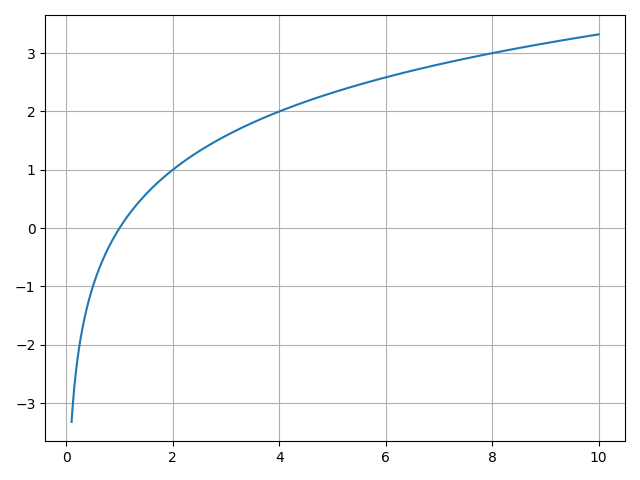
\includegraphics[width=\columnwidth]{figs/1_6_1.png}
        \caption{$h(X)$ as a function of $a$.}
        \label{fig:1-6-1}
    \end{figure}
\end{enumerate}
\end{document}